\section{Confronto veicolo Ego Simulato e Reale}
\subsection{Accelerazione}
\paragraph{Premessa}
Come anticipato nella Sottosezione \ref{subsec:ego_acceleration}, in Figura \ref{fig:acceleration_effettiva_impartita} 
viene confrontata l'accelerazione \textbf{impartita} (linea gialla) dal sistema di controllo adattivo della velocità (ACC) 
con l'accelerazione \textbf{effettiva} (linea viola) del veicolo \emph{ego} misurata nella realtà.  
Il valore dell'accelerazione impartita corrisponde alla colonna \texttt{ACC command acceleration} del \texttt{dataset\_reale}, 
mentre l'accelerazione effettiva è stata calcolata come:
\[
a_t(\mathrm{ego}) = \frac{v_t(\mathrm{ego}) - v_{t-1}(\mathrm{ego})}{\Delta t}
\]
a partire dalla colonna \texttt{ego\_velocity} del \texttt{dataset\_reale}.
\begin{figure}[H]
    \centering
    \adjustbox{center}{
        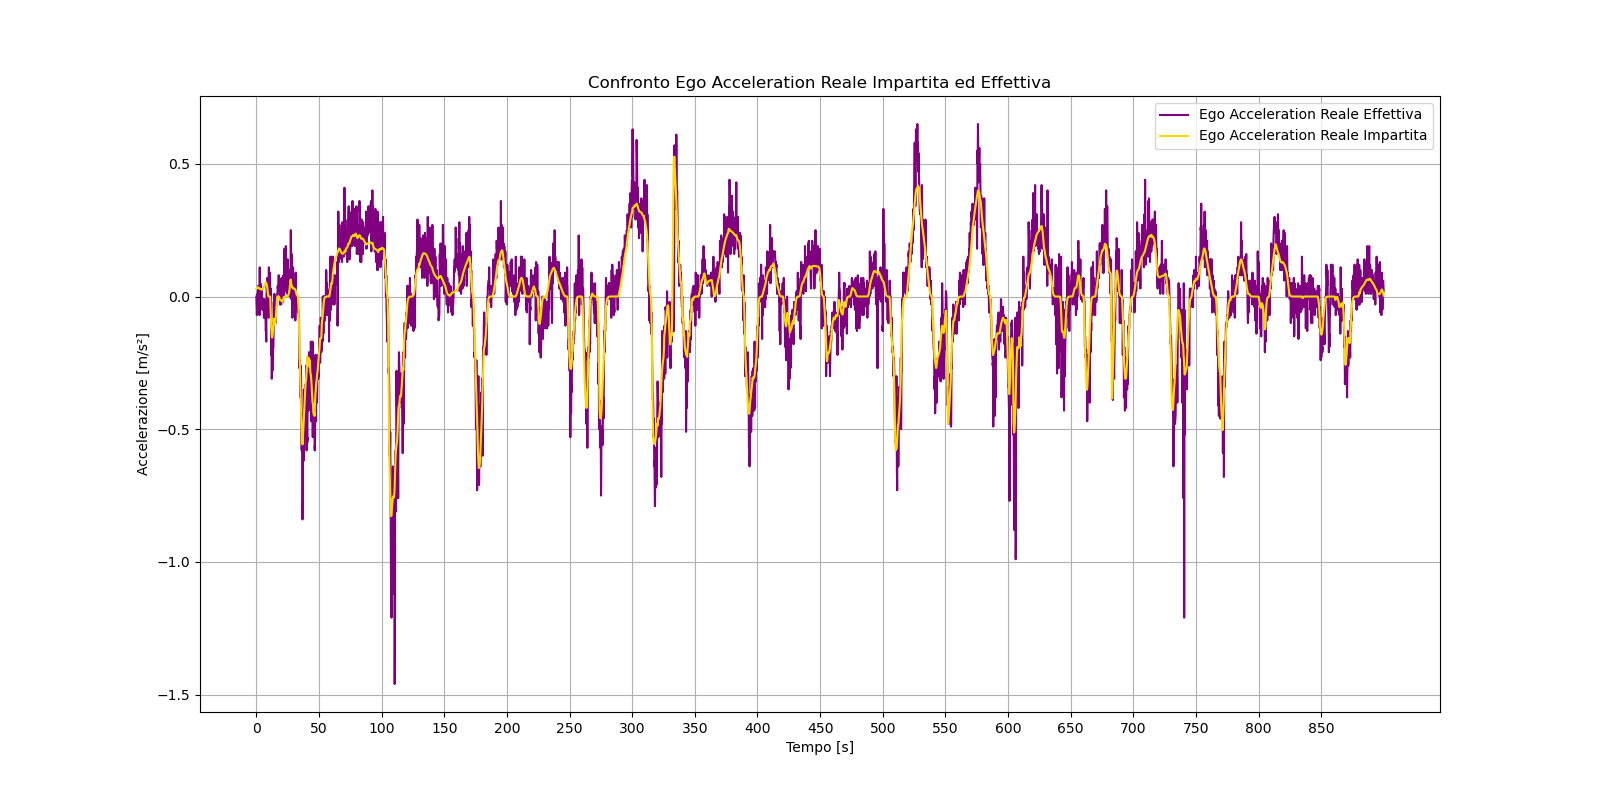
\includegraphics[width=1.25\linewidth]{simulation/real_data_comparison/acceleration_effettiva_impartita.png}
    }
    \caption{Confronto Ego Acceleration Reale Impartita ed Effettiva}
    \label{fig:acceleration_effettiva_impartita}
\end{figure}
\noindent Il grafico evidenzia una discrepanza significativa tra i due segnali.  
In particolare, l'accelerazione impartita mostra variazioni più regolari e smussate, mentre l'accelerazione effettiva presenta un andamento 
notevolmente più irregolare e “rumoroso”.  
Questa differenza riflette le dinamiche reali del veicolo, che impediscono di replicare istantaneamente e in modo perfettamente fedele 
i comandi teorici dell'ACC.  
Tale comportamento è influenzato da diversi fattori, tra cui i ritardi nella risposta del motore o del sistema frenante 
e le caratteristiche meccaniche del veicolo.
\\\\
\noindent Come già discusso, in questa analisi si è adottata la semplificazione di assumere l'accelerazione impartita dal modello 
uguale a quella effettiva.  
Va tuttavia sottolineato che questa approssimazione comporta inevitabilmente un calcolo della \emph{ego\_velocity} non perfettamente corrispondente alla realtà.  
Nonostante ciò, l'ipotesi è ritenuta accettabile per la valutazione delle performance complessive del sistema.
\begin{figure}[H]
    \centering
    \adjustbox{center}{
        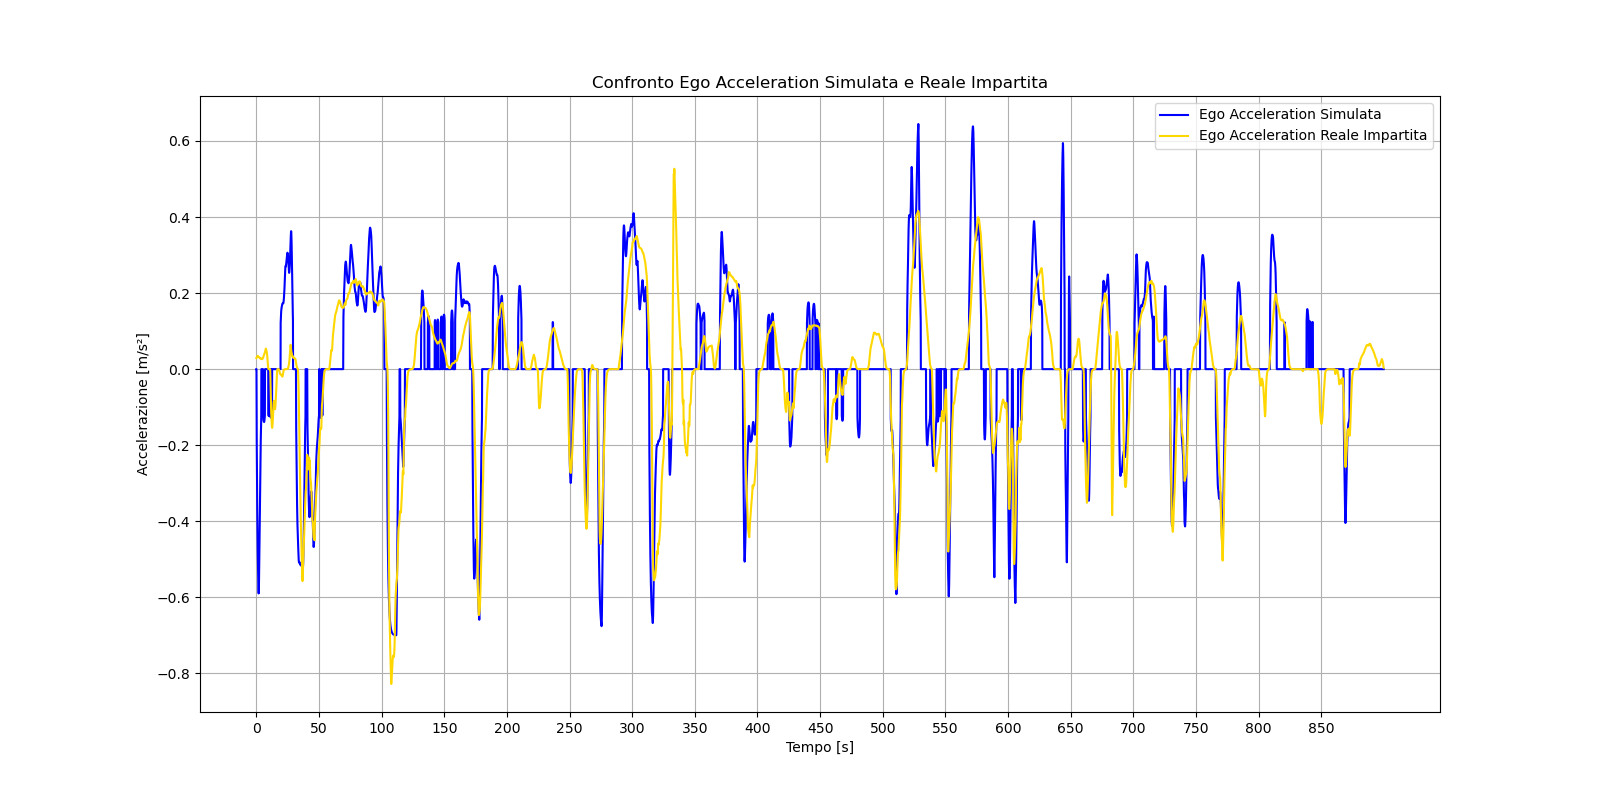
\includegraphics[width=1.25\linewidth]{simulation/real_data_comparison/acceleration_impartita.png}
    }
    \caption{Confronto Ego Acceleration Simulata e Reale Impartita}
    \label{fig:acceleration_impartita}
\end{figure}
\begin{figure}[H]
    \centering
    \adjustbox{center}{
        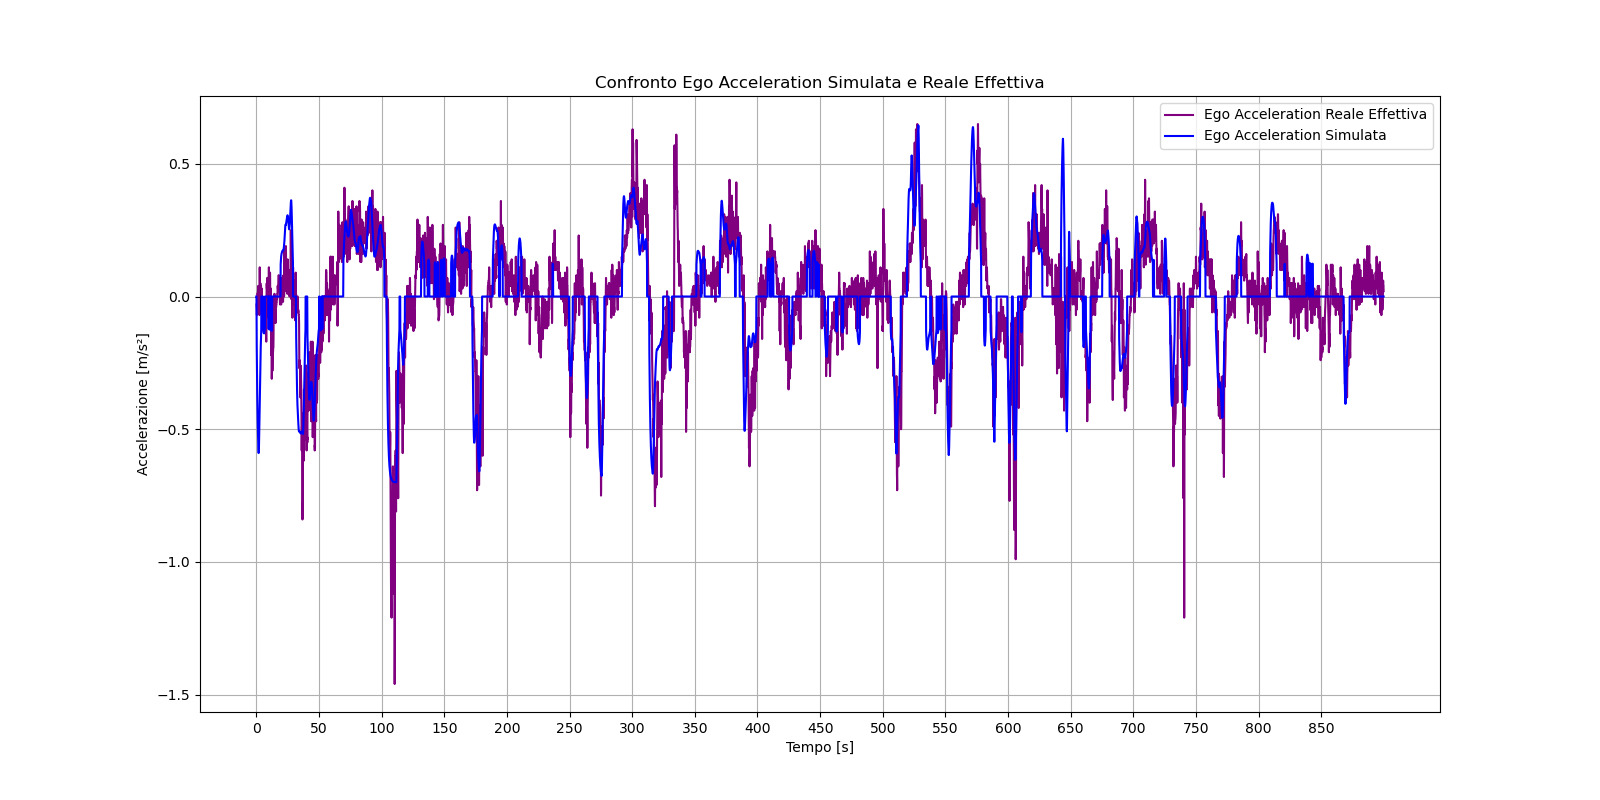
\includegraphics[width=1.25\linewidth]{simulation/real_data_comparison/acceleration_effettiva.png}
    }
    \caption{Confronto Ego Acceleration Simulata e Reale Effettiva}
    \label{fig:acceleration_effettiva}
\end{figure}
\subsection{Velocità}
\begin{figure}[H]
    \centering
    \adjustbox{center}{
        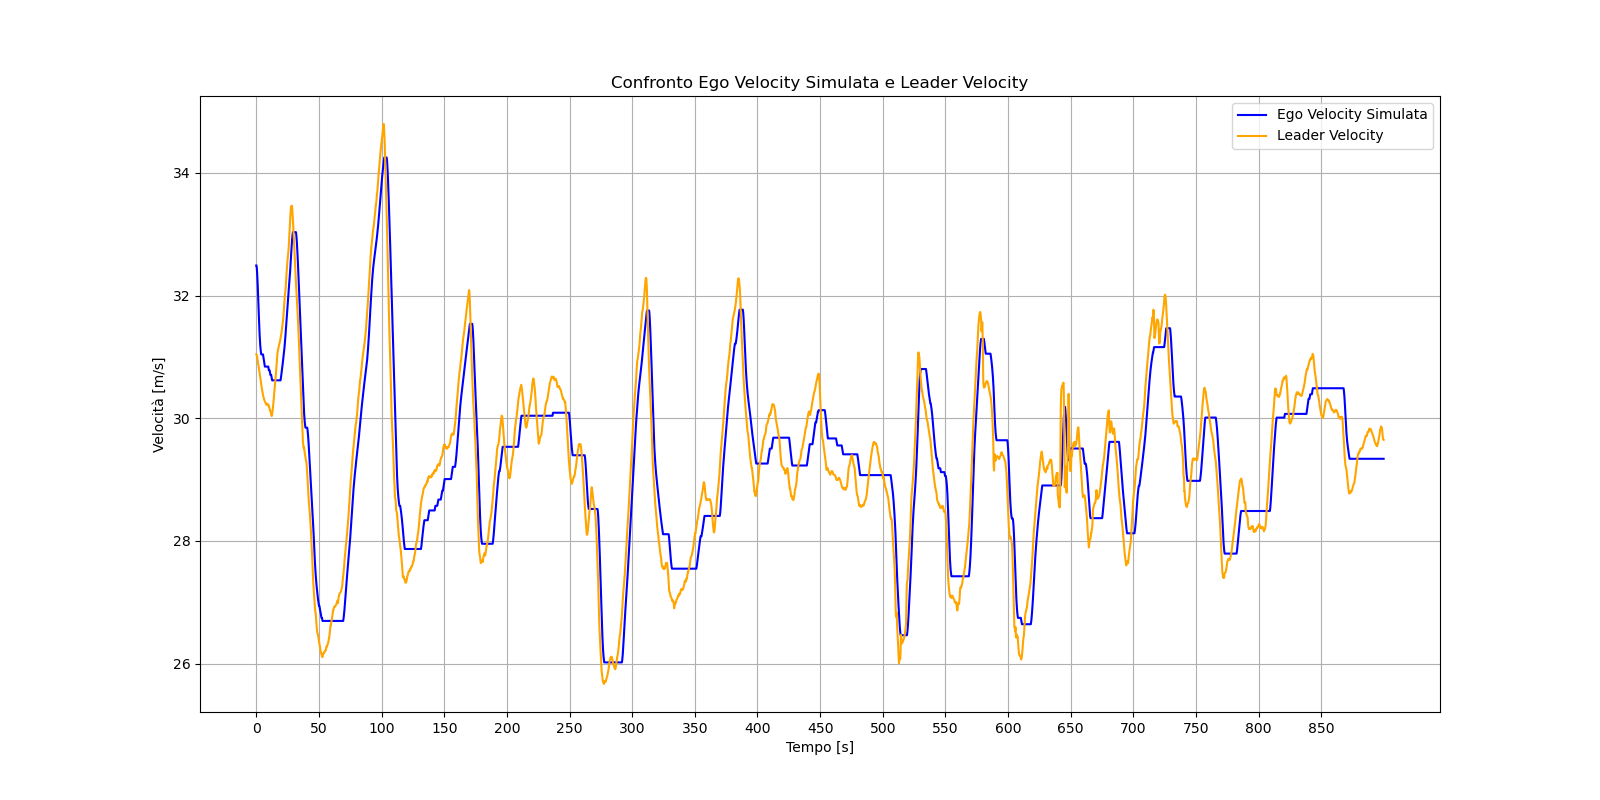
\includegraphics[width=1.25\linewidth]{simulation/real_data_comparison/velocity.png}
    }
    \caption{Confronto Ego Velocity Simulata e Reale}
    \label{fig:ego_velocity_reale}
\end{figure}
